\begin{figure*}[t]
\centering
    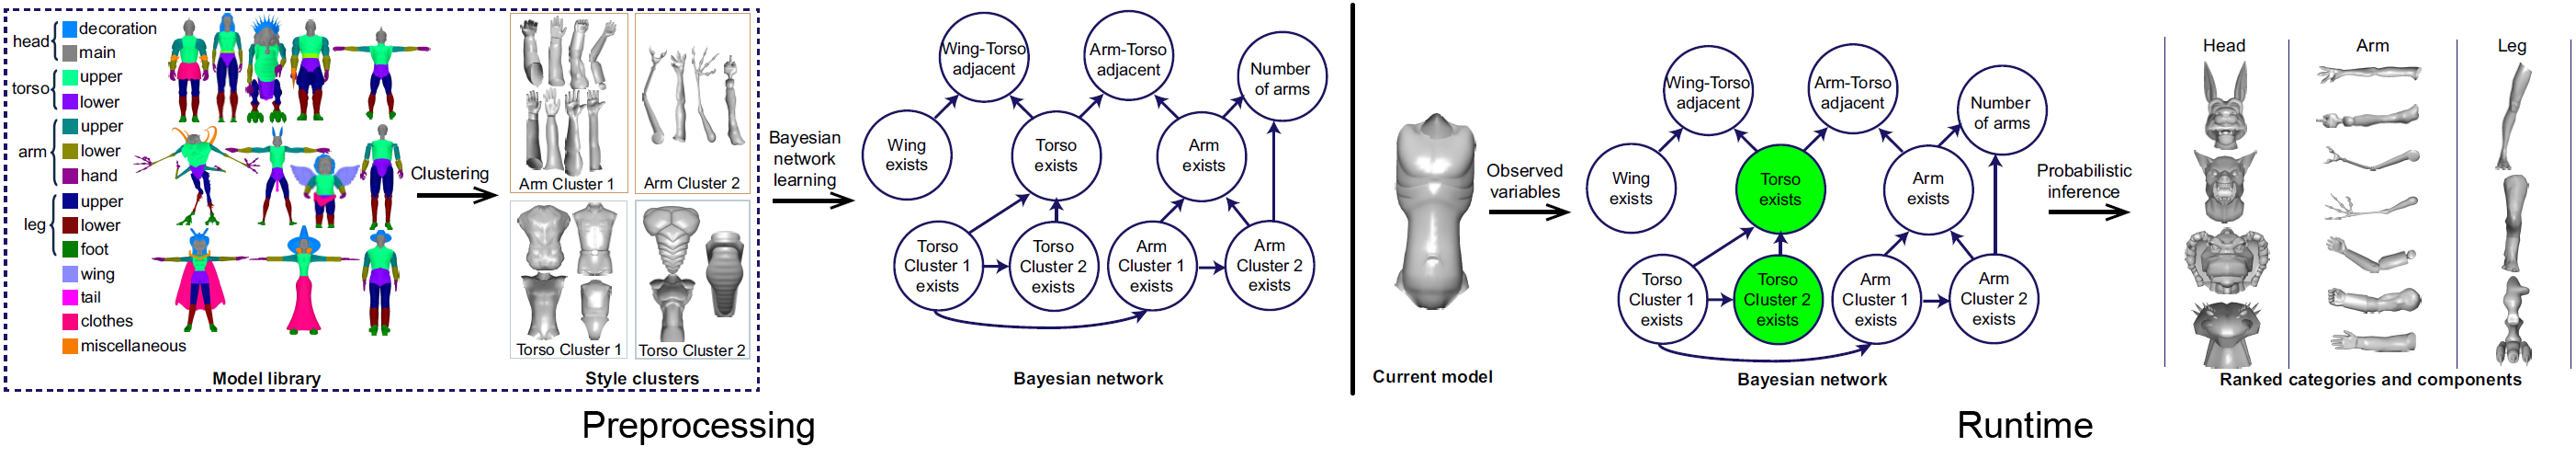
\includegraphics[width=1.0\linewidth]{fig/img/chaudhuri_sig11_prob.png}
    %\vspace{-0.4cm}
    \caption{
    Given a library of models, a Bayesian network encoding semantic and geometric relationships among shape parts
    is learned~\cite{Chaudhuri:2011:prabm} (top). The modeling process (bottom) performs probabilistic inference in the learned
    Bayesian network to generate ranked lists of category labels and components within each category, customized for the currently assembled model.}
    \label{fig:segmentation_labeling}
\end{figure*}

